\documentclass[11pt]{article}
%%%
% TODO TOM: Add theory and motivation intro
%% Finish smoothing comparison
%% Comment code    


%% TODO MAREK: Results/conclusion
%%  Language check

%%%
%% Separate file for preamble with macros and stuff
\usepackage[T1]{fontenc}
\usepackage[a4paper, top=1in, bottom=1.1in, left=1in, right=1in]{geometry}
\usepackage[toc,page]{appendix}
\usepackage[utf8]{inputenc} % utf8
\usepackage{amsmath}
\usepackage{attachfile}
\usepackage{booktabs}
\usepackage{caption}
\usepackage{commath}
\usepackage{graphicx}
\usepackage{hyperref}
\usepackage{listings}
\usepackage{mathtools}
\usepackage{siunitx}
\usepackage{subcaption}
\usepackage{tabularx}
\usepackage{url}
\usepackage{varioref}
\usepackage{wrapfig}
\usepackage{xcolor}

\setlength{\belowcaptionskip}{-6pt}
\makeatletter
\lst@Key{matchrangestart}{f}{\lstKV@SetIf{#1}\lst@ifmatchrangestart}
\def\lst@SkipToFirst{%
  \lst@ifmatchrangestart\c@lstnumber=\numexpr-1+\lst@firstline\fi
  \ifnum \lst@lineno<\lst@firstline
  \def\lst@next{\lst@BeginDropInput\lst@Pmode
    \lst@Let{13}\lst@MSkipToFirst
    \lst@Let{10}\lst@MSkipToFirst}%
  \expandafter\lst@next
  \else
  \expandafter\lst@BOLGobble
  \fi}
\makeatother

\lstset{  
  backgroundcolor=\color{gray!30},   % choose the background color; you must add \usepackage{color} or \usepackage{xcolor}
  basicstyle=\scriptsize,        % the size of the fonts that are used for the code
  breakatwhitespace=false,         % sets if automatic breaks should only happen at whitespace
  breaklines=true,                 % sets automatic line breaking
  captionpos=t,                    % sets the caption-position to bottom
  escapeinside={\%*}{*)},          % if you want to add LaTeX within your code
  extendedchars=true,              % lets you use non-ASCII characters; for 8-bits encodings only, does not work with UTF-8
  frame=single,                   % adds a frame around the code
  keepspaces=true,                 % keeps spaces in text, useful for keeping indentation of code (possibly needs columns=flexible)
  keywordstyle=\color{blue},       % keyword style
  language=C++,                 % the language of the code
  numbers=left,                    % where to put the line-numbers; possible values are (none, left, right)
  numbersep=20pt,                   % how far the line-numbers are from the code
  numberstyle=\tiny\color{gray}, % the style that is used for the line-numbers
  rulecolor=\color{blue!20},       
  showspaces=false,                % show spaces everywhere adding particular underscores; it overrides 'showstringspaces'
  showstringspaces=false,          % underline spaces within strings only
  showtabs=false,                  % show tabs within strings adding particular underscores
  stepnumber=1,                    % the step between two line-numbers. If it's 1, each line will be numbered
  tabsize=2,                   % sets default tabsize to 2 spaces
  framesep=7pt,
  xleftmargin=12pt,
  xrightmargin=11pt
}


\setlength{\fboxsep}{4pt}
\DeclareCaptionFormat{myformat}{%
  \hspace{1pt}\fcolorbox{blue!20}{gray!20}{\footnotesize\parbox{\dimexpr\textwidth-17pt\relax}{#1#2\ttfamily#3}}\vspace{-4pt}
}
\captionsetup[lstlisting]{format=myformat}

\captionsetup[figure]{labelfont=sf,hypcap=false,format=hang,margin=0.5cm,justification=RaggedRight,calcwidth=0.7\linewidth,font=footnotesize,justification=justified}
\captionsetup[subfigure]{labelfont=sf,hypcap=false,format=hang,margin=0.5cm,justification=RaggedRight,calcwidth=0.7\linewidth,font=footnotesize,justification=justified}
\captionsetup[table]{labelfont=sf,hypcap=false,format=hang,margin=1cm,justification=RaggedRight,calcwidth=0.8\linewidth,font=footnotesize,justification=justified}
\labelformat{equation}{(#1)}

%%% Math typesetting macros
\newcommand{\di}[2]{#1_\textup{#2}} % Descriptive Index: Macro for quick upright index (as opposed to a variable index, which should be italic)


\renewcommand{\lstlistlistingname}{Code listings}
\bibliographystyle{ieeetr}


%%%%%%%%%%%%%%%%%%%%%%%%%%%%%%
%%% STOLEN FROM STACKOVERFLOW
%%%%%%%%%%%%%%%%%%%%%%%%%%%%%%

\newcommand\YAMLcolonstyle{\color{red}\mdseries\scriptsize}
\newcommand\YAMLkeystyle{\color{black}\bfseries\scriptsize}
\newcommand\YAMLvaluestyle{\color{blue}\mdseries\scriptsize}

\makeatletter

% here is a macro expanding to the name of the language
% (handy if you decide to change it further down the road)
\newcommand\language@yaml{yaml}

\expandafter\expandafter\expandafter\lstdefinelanguage
\expandafter{\language@yaml}
{
  keywords={true,false,null,y,n},
  keywordstyle=\color{darkgray}\bfseries,
  basicstyle=\YAMLkeystyle,                                 % assuming a key comes first
  sensitive=false,
  comment=[l]{\#},
  morecomment=[s]{/*}{*/},
  commentstyle=\color{purple}\ttfamily,
  stringstyle=\YAMLvaluestyle\ttfamily,
  moredelim=[l][\color{orange}]{\&},
  moredelim=[l][\color{magenta}]{*},
  moredelim=**[il][\YAMLcolonstyle{:}\YAMLvaluestyle]{:},   % switch to value style at :
  morestring=[b]',
  morestring=[b]'',
  literate =    {---}{{\ProcessThreeDashes}}3
  {>}{{\textcolor{red}\textgreater}}1
  {|}{{\textcolor{red}\textbar}}1
  {\ -\ }{{\mdseries\ -\ }}3,
}

% switch to key style at EOL
\lst@AddToHook{EveryLine}{\ifx\lst@language\language@yaml\YAMLkeystyle\fi}
\makeatother

\newcommand\ProcessThreeDashes{\llap{\color{cyan}\mdseries-{-}-}}


\renewcommand{\tabularxcolumn}[1]{>{\small}m{#1}}
%%% Local Variables:
%%% mode: latex
%%% TeX-master: t
%%% End:


%% For make-title
\title{Laboration 2: RGBD-cameras\\ {\small Sensors and Sensing}} \author{Marek
  Bečica, Tom Olsson} \date{\today}

\begin{document}
\maketitle %Title area
\begin{center}
  \emph{All code for this exercise can be found at \\ \url{https://github.com/tgolsson/sensors-laboration2-xtion}}\\
  \textbf{\large In some of the plots the variance is wrongly labeled as
    ``staider''. This is just a typesetting error in the images, and not the
    actual values. All values used are variances.}
\end{center}
\tableofcontents
\lstlistoflistings % List of all code snippets
\listoffigures % List of all figures
\listoftables \lstset{
  matchrangestart=t} %initialise the linerange-macro for \lstinput...
\section{Theory and motivation}


\subsection{RGBD-cameras}
RGBD-cameras, short for \emph{Red-Green-Blue-Depth}-camera, is a type of
low-cost camera commonly used for robot vision. The concept became widely
popular with the release of the Microsoft Kinect in late 2010. \par

These cameras consist of two separate parts: one normal color-based camera, and
one infra-red sensor with accompanying projector. The sensing consists of
projecting a deterministic pattern onto the scene using an infrared emitter, and
then unprojecting by comparing the image to previously captured patterns at
known depths. By interpolating through these patterns, a full depth-image is
generated.


\subsection{Noise}

A common problem in any type of sensing is the introduction of noise into the
system. This noise can come from many sources, and be predictable or
unpredictable. Examples of noise sources could be frequency hum from electric
circuits, flickering lights, air pollution or pure inaccuracy. This noise can
skew the results of sensors that make algorithm much more error prone. \par

There are many approaches to reduce noise. Proper calibration and good testing
environments is a good start, but this can only reduce external noise. Internal
noise of the sensor needs to be analyzed and minimized on a much lower-level
such as by using specially constructed algorithms. For sensors that generate
some sort of sequence, one very naive (but nonetheless effective) approach is
the use of smoothing. \par

\section{Implementation}
The purpose of this exercise is to calibrate an RGBD-camera and investigate its
characteristics. Then, several smoothing algorithms shall be evaluated to reduce
noise in the depth sensor.

\subsection{Hardware and environment}
This exercise was performed using an \emph{ASUS Xtion Pro}. The camera was
connected over \emph{USB2} to a laptop running Linux kernel 4.2.5. The
communication to the camera is done using the \emph{Robot Operating System}
[ROS] version \emph{Indigo Igloo}. All ROS packages used are compiled directly
from GitHub development branch for Indigo Igloo. \par
Other software used includes the OpenCV libraries, version 2.4.12.2-1.

\subsection{Camera setup}
As a first step we had to install \emph{openni2} package for the corresponding
version of ROS. This package contains drivers for the ASUS camera. After
installing the package we connected the camera to the USB 2.0 port on the
laptop. We made sure that our system can recognize the camera through command
\texttt{lsusb} and after that we run the openni2 package using \texttt{roslaunch
  openni2\_launch openni2.launch}. \par
During the first launch there was a warning about no calibration file found, but
we didn't need it yet for the camera testing. After running openni2 we run in
the new terminal window command \texttt{rosrun rviz rviz}, which we used for
inspecting the topics where camera publishes its data. In the RVIZ window we
needed to set global option \textbf{Fixed Frame} to \textbf{camera\_link} in
order to see the camera data. \par

We need to create several visualizations to see what camera publishes on each
topic. There are four major types of topics with different subtopics that can be
visualized using RVIZ. There are topics for \textbf{depth image}, \textbf{depth
  registered image}, \textbf{RGB image} and \textbf{infrared image}. From the
depth and depth registered topic we can also get point cloud. The topics can be
seen in table \vref{tab:table1} (we omitted the subtopics, because they contains
the same data, but with different compress method, which is not relevant for
this task). \par
\noindent
{
  \begin{tabularx}{1\textwidth}{lXc}
  
      \toprule
      Topic & Description & Data preview\\
      \midrule
      \texttt{/camera/depth/image\_raw} &
      Contains depth image & 
\raisebox{-.5\height}{      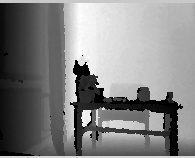
\includegraphics[width=0.2\textwidth]{figures/depth-image-raw.png}}\\
      
      \texttt{/camera/depth/points} &
      Contains point cloud of the point distances & 
\raisebox{-.5\height}{      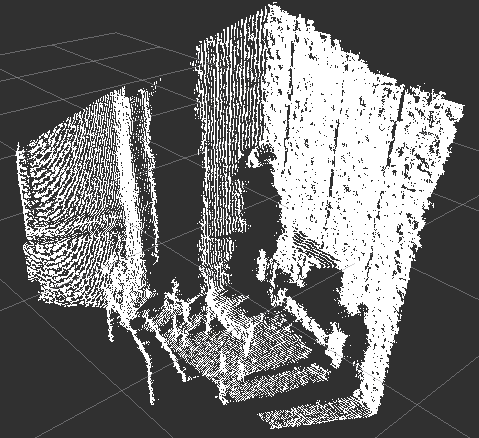
\includegraphics[width=0.2\textwidth]{figures/depth-image-raw-pointcloud.png}}\\
      
      \texttt{/camera/depth\_registered/image\_raw} &
      Contains depth image projected from both sensors& 
\raisebox{-.5\height}{      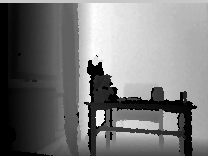
\includegraphics[width=0.2\textwidth]{figures/depth_registered-image-raw.png}}\\
      
      \texttt{/camera/depth\_registered/points} &
      Contains point cloud of the point distances projected from both sensors & 
\raisebox{-.5\height}{      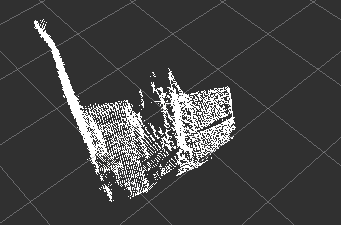
\includegraphics[width=0.2\textwidth]{figures/depth_registered-image-raw-pointcloud.png}}\\
      
      \texttt{/camera/ir/image} &
      Contains infrared image & 
\raisebox{-.5\height}{      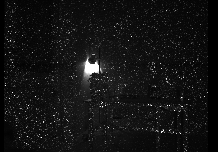
\includegraphics[width=0.2\textwidth]{figures/ir-image-raw.png}}\\
      
      \texttt{/camera/rgb/image\_raw} &
      Contains RGB image & 
\raisebox{-.5\height}{      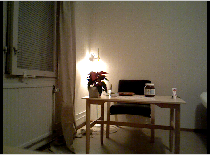
\includegraphics[width=0.2\textwidth]{figures/rgb-image-raw.png}}\\
      \bottomrule
    \end{tabularx}
    \captionof{table}[ROS: Camera topics]{\label{tab:table1}Camera ROS topics}
  }



\subsection{ROS setup}
Instead of using RVIZ to view the data as before, a custom ROS-node can be
used. As there are three types of data, color image, depth image, and point
cloud, there are three listeners setup to receive this data. An example of the
data on these topics can be found in the embedded files below\footnote{If these
  embedded files do not work, such as if you use Adobe Acrobat, please download
  them from the \texttt{report} folder in the GitHub repository. Verified to
  work with Okular and Evince on Linux.}. The \texttt{depth image} and
\texttt{color image} are stored in the OpenCV \texttt{y[a]ml} format, and the
point cloud is stored in the \emph{Point Cloud Library} [PCL] \texttt{pcd}
format.\par

\begin{center}
  \attachfile[color=0 0 0,icon=Paperclip]{pcloud.pcd}{{ }Point cloud file}{ }
  \attachfile[color=0 0 0,icon=Paperclip]{rgbbmp.yml}{{ }RGB-image file}{ }
  \attachfile[color=0 0 0,icon=Paperclip]{rgbdepth.yml}{{ }Depth-image file}
\end{center}

\subsection{Camera calibration}

In this part we were supposed to calibrate the camera which requires to setup
internal parameters. After that we should be able to get not distorted image
from the camera and right distance measurement. \par

As a first step we had to install \emph{camera\_calibration} package. After that
we listed all topics where camera publishes its data and we chose topic
\texttt{/camera/rgb/image\_raw}. Before running the calibration process, we
measured the number of squares on the checkerboard and their size. Using the
command \texttt{rosrun camera\_calibration cameracalibrator.py --size=6x10
  --square=0.065 image:=/camera/rgb/image\_raw}{ } \texttt{camera:=/camera/rgb
  --approximate=0.1}, we run the calibration application with correctly setup
parameters according to our measurements of the calibrating pattern. \par

In the calibration window we could see image from the selected topic with
detection of the pattern. We set the camera to the parallel position with the
ground and pointed it to the wall. After that we kept moving and tilting the
pattern all over the camera field of view until X, Y and Size progress bar
showed long line and button Calibrate light up. This process took up about 2
minutes until we got good results and Calibration button lighted up. We pressed
the button and then waited for few minutes until the application was able to
compute the right parameters for our camera. After that buttons Save and Upload
lighted up. We saved the calibration file and tried to upload it to the camera
firmware, but for some reason that function didn't worked properly and we had to
set the calibration file as a parameter of the openni2 package. \par
        
The calibration file was saved into \emph{out.txt} file in the \textbf{tmp}
directory and we needed to convert it to YAML file. In order to do that, we used
command \texttt{rosrun camera\_calibration\_parsers convert out.txt camera.yaml}
which converted the calibration file into yaml file which we could use for the
openni2 package. The calibration file is shown in listing \vref{lst:calib}. \par
        
To check the calibration results we pointed the camera at some straight lines
(wall corners, table etc.) and checked if they got distorted around the
edges. That showed that the straight lines stayed as straight lines, so the
calibration was successful. To quantitatively verify if the calibration worked
we run the code from the Task 4: Noise characterization, that measured average
and standard deviation for the distance in the small window. Then we pointed the
camera to the objects in different distances and checked if the mean of the
distance is the same as the reality, which mostly was within the range of the
camera. \par
	
\lstinputlisting[language=yaml,caption={The calibration file for the camera},
label={lst:calib}]{camera.yaml}

\subsection{Noise characterization}

The sensors used in the camera suffer from noise, and the first requirement for
improvement is to objectively quantify the error. First, 5 measurements of 10
seconds each were recorded with \texttt{rosbag}. The measurements were taken
\emph{50}, \emph{100}, \emph{150}, \emph{200}, and \emph{300} cm from a white
wall. The camera was placed on a table, so that the camera normal was
perpendicular to the wall. This ensures that all later noise and smoothing
comparisons are made against the same baseline. \par

First, the errors were quantified at varying distance with set window
sizes. Fig. \vref{fig:20x20} shows the error and variances for a 20x20 window,
and fig. \vref{fig:40x40} shows the same for a 40x40 window. The most obvious
pattern can be seen in the right-most plot in the two figures: there is a very
strong correlation between distance and both variance and error. This has been
shown by other researchers, and is logical: the further the distance, the more
things can interfere with measurements such as light conditions, dust particles,
and so on. \par

Another interesting pattern is that the mean error barely changes between the
two windows; however, a larger window reduces the variance significantly. This
is not so much related to reduced errors, but a result of the definition of a
variance. If the errors are assumed to adhere to some sort of distribution
$X \in \left(-\infty, \infty \right)$, then $\sum_{X_1}^{X_\infty} = \bar{X}$,
i.e., the static error. From this it follows that the variance will then also be
on same order of magnitude as the noise in the signal. However, if too few
points are sampled the sum will only approximate the mean, and the variance will
become unstable. There is therefore a trade-off between window size and
computational cost; i.e. while a larger window may be preferable for preciseness this may be
computationally expensive, especially for more complex filters. \par

\begin{figure}[ht]
  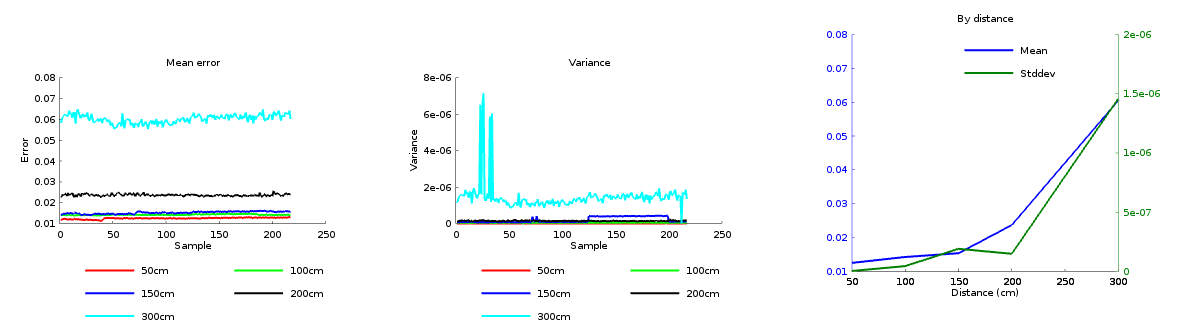
\includegraphics[width=1\textwidth]{figures/20x20-plot.png}
  \captionof{figure}[Mean and variance: 20x20 window]{\label{fig:20x20} The
    error and variance for a 20x20 pixel window at the center.}
\end{figure}

\begin{figure}[ht]
  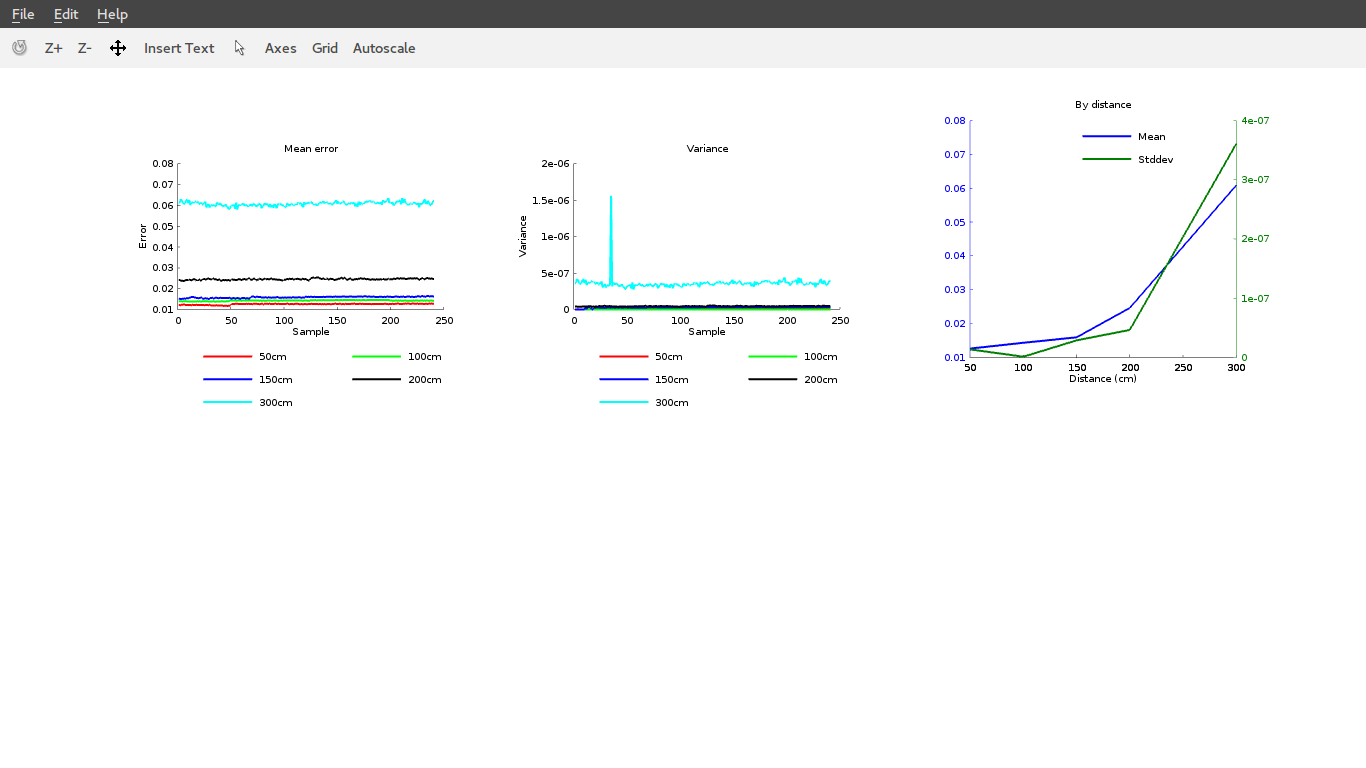
\includegraphics[width=1\textwidth]{figures/plot40x40.png}
  \captionof{figure}[Mean and variance: 40x40 window]{\label{fig:40x40} The
    error and variance for a 40x40 pixel window at the center.}
\end{figure}

Moving on, the distance can instead be kept constant while the window size is
varied. This is shown for 50 cm in fig.  \vref{fig:variedwindow}. Here, the
effect mentioned above with variance is amplified a lot; and error and variance
become very stable for the large window sizes; and in the case of variance also
very small. There is a visible artifact between samples 0-60 which
has much smaller values than the other values. As most of the values are higher, these
smaller values can be discarded. \par


\begin{figure}[ht]
  \centering
  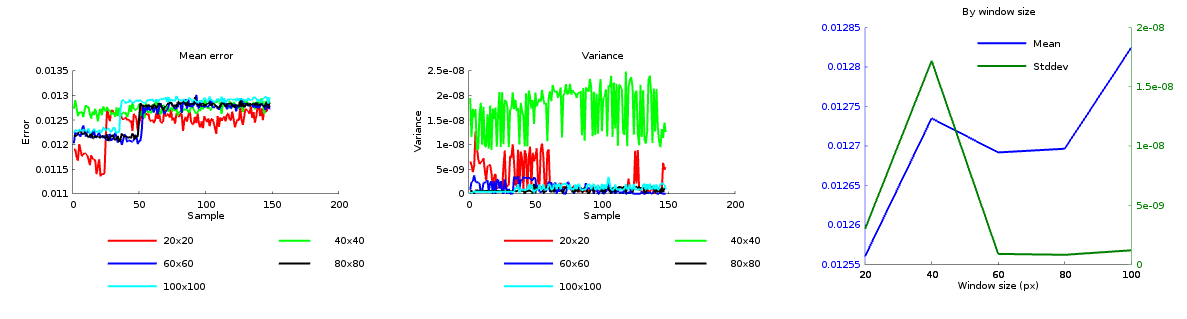
\includegraphics[width=1\textwidth]{figures/plotwindowsizes.png}
  \captionof{figure}[Mean and variance: 50 cm, varied window
  sizes]{\label{fig:variedwindow} The error and variance at 50 cm for various
    window sizes.}
\end{figure}

The cleaned data shown in fig. \vref{fig:variedwindow2} highlights how stable
the mean is for the larger window sizes. It also shows that something is
interfering in the 40x40 measurement, though it is hard to pinpoint what. One
(hypothetical) possibility is that there is a small patch of very noisy values
that get introduced when the window size increases, and as the window size is
still quite small it has a large impact on the variance. \par

One last conclusion can be seen, and this is that the mean increases with window
sizes. This is caused by the increase in angle towards the edges of the
window. As all distances are measured from the sensor, this causes them to
increase slightly. The increase is approximately $\frac{1}{\cos \alpha}$, where
$\alpha$ is the angle relative to the camera normal.\par

\begin{figure}[ht]
  \centering
  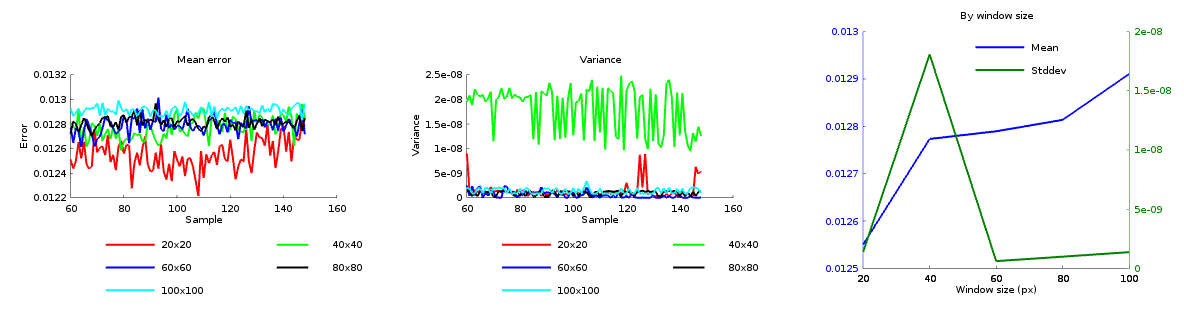
\includegraphics[width=1\textwidth]{figures/plot2bywindowsize.png}
  \captionof{figure}[Mean and variance: 50 cm, varied window sizes,
  cleaned]{\label{fig:variedwindow2} The error and variance at 50 cm for various
    window sizes with faulty data removed.}
\end{figure}

\subsection{Noise filtering}

To improve the input depth image five different filters were implemented for
smoothing. The first three filters; \emph{median}, \emph{gaussian}, and
\emph{bilateral}, come from the OpenCV library. The last two filters, in the
temporal domain, were implemented manually in C++ and are shown in listing
\vref{lst:temporal}. A large issue when using the filters was handling the large
number of invalid values in the input. In some situations, a majority of the
elements were NaN, which obviously makes it hard to draw any conclusions from
the data. This caused particular problems with the bilateral filter, which
suffers a segmentation fault when there are too many NaN values in the
input. \par

\lstinputlisting[float,caption={The temporal smoothing
  algorithm},label={lst:temporal},language=C++,linerange={240-277}]{../asus_node/src/asus_node.cc}


In order to solve this issue, all NaN-values in the input are set to $10000$
before being passed to the bilateral filter. By the edge preserving property of
bilateral filtering, this should reduce the impact they have on the actual
filtering process. After the filtering is done, every cell which was set to 10
000 is set to 0; and the mean and variance is calculated on all non-zero
elements. \par

Another solution we considered - but did not implement - was to use local
median-filtering at each \texttt{NaN}. We deemed this to be a very computationally
expensive process, but could possibly yield better results. \par

The result of filtering our depth-images is seen below in
fig. \ref{fig:plots20x20filtered} and \vref{fig:plots40x40filtered}. Just as in
the previous section, the unreliable data at the start is removed to clean up
the results.

\begin{figure}[ht]
  \centering
  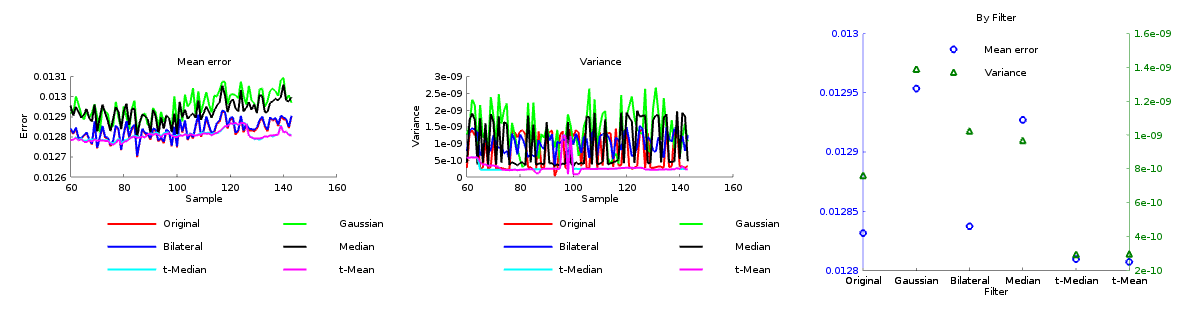
\includegraphics[width=1\textwidth]{figures/plot20x20filtered.png}
  \captionof{figure}[Filtered data: 20x20, 50 cm]{\label{fig:plots20x20filtered}
    Mean and variance for the filters at 50 cm with 20x20 window size.}
\end{figure}
\begin{figure}[ht]
  \begin{center}
    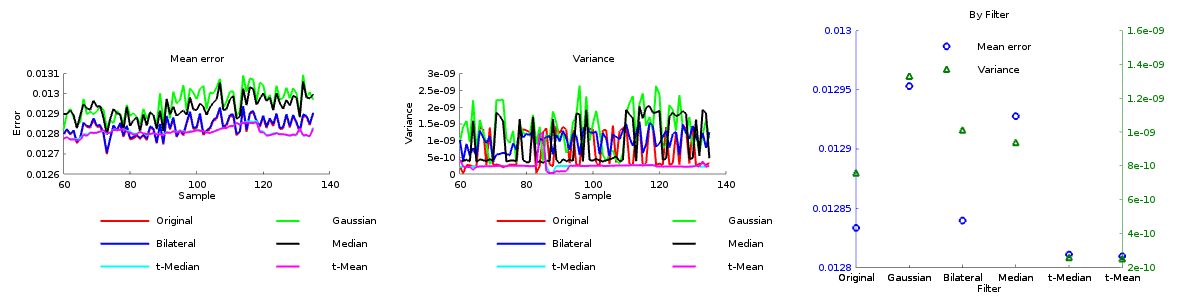
\includegraphics[width=1\textwidth]{figures/plot40x40filtered.png}
    \captionof{figure}[Filtered data: 40x40,
    50 cm]{\label{fig:plots40x40filtered} Mean and variance for the filters at 50
      cm with 40x40 window size.}
  \end{center}
  

\end{figure}

To visualize the smoothing algorithms we set up a scene with a small box in the middle, and a bigger box behind it. This allowed us to clearly see the edges of the smaller box through the camera. As we can see in the original
image (fig. \vref{fig:refimage}) there is a lot of noise and the edges are not as clear
as they should be. The used filters should smooth out the noise to be able to
get better measurements. The resulting image \vref{fig:filterswindow} shows all
filters applied to the center of the image. \par

The first image is the original window 80x80 px without any filters applied but
we removed NaN values and replaced them with high number. Second image is
original with applied gaussian blur filter. This filter blurs the image and
reduce details, which results in smoother edges and reduced noise. Third picture
is image with applied median filter. We can see that median filter preserves the
edges while removing some noise. \par

First picture in the second row is original image with applied bilateral
filter. This filter also preserves sharp edges and removes some noise by
smoothing the image. The second picture in the same line is the average over 10
images. That method can reduce some noise, which appears only in few pictures or
reduce effect of moving objects, that could affect the measurements. Last
picture is the median over 10 images. Effect of that method is similar
to the previous one, but it preserves more details.

\begin{figure}[ht]
  \centering
  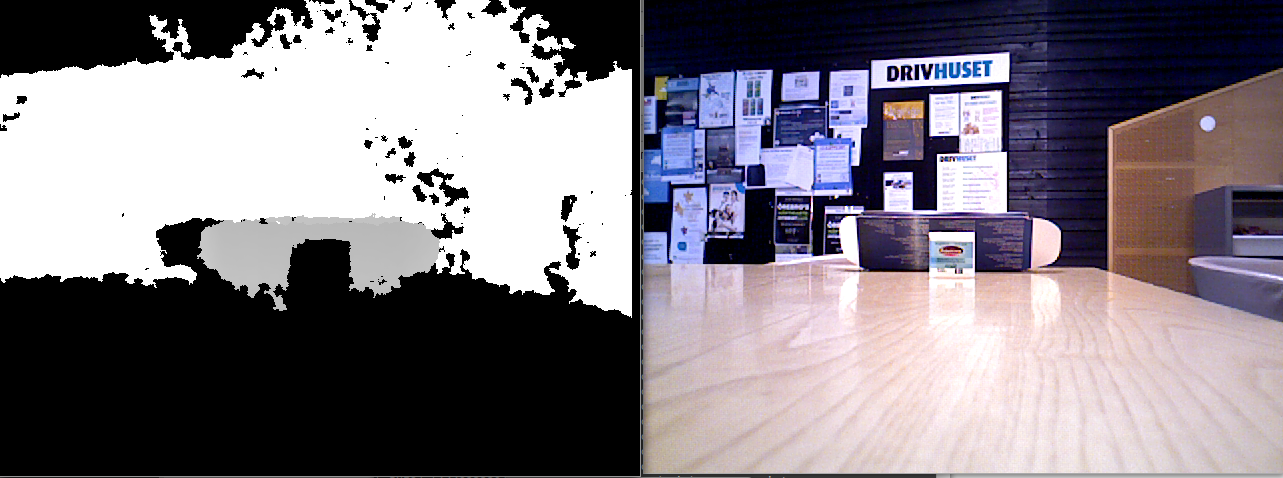
\includegraphics[width=1\textwidth]{figures/reference_rgb_depth.png}
  \captionof{figure}[Reference scene: RGB and depth
  image]{\label{fig:refimage} Reference image for demonstrating effects of the
    filters}
\end{figure}
\begin{figure}[ht]
  \centering
  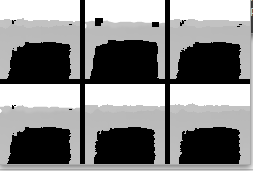
\includegraphics[width=1\textwidth]{figures/applied_filters_center.png}
  
  \captionof{figure}[Reference scene: Filtered 80x80 center
  window]{\label{fig:filterswindow} This image shows different filters applied
    to the center of the window 80x80 px. From the top left corner - original
    image, gaussian, median, bilateral, temporal average, temporal median}
\end{figure}

\section{Results}
% Both : Summary...

\bibliography{References}
\end{document}



%%% Local Variables:
%%% mode: latex
%%% TeX-master: t
%%% End:
